\section{9. Marketing Plan}

\subsection*{Budget Allocation (€150,000)}

\begin{itemize}
    \item \textbf{Digital Ads (40\%):}
    \begin{itemize}
        \item Google Ads targeting “EV charging near me.”
        \item LinkedIn campaigns for fleet operators.
    \end{itemize}
    \item \textbf{Partnerships (30\%):}
    \begin{itemize}
        \item Co-marketing with automakers (Renault, VW).
        \item Free charging weekends at partnered malls.
    \end{itemize}
    \item \textbf{Content (20\%):}
    \begin{itemize}
        \item YouTube tutorials (“How to charge in 20 mins”).
        \item Blog series on sustainability (e.g., “Solar + EVs = Zero Emissions”).
    \end{itemize}
    \item \textbf{Events (10\%):}
    \begin{itemize}
        \item Sponsorship of EU Green Mobility Summit.
    \end{itemize}
\end{itemize}

\subsection*{KPIs}
\begin{itemize}
    \item 5,000 app downloads (Q1).
    \item 20\% conversion rate from free to paid users.
    \item 15+ municipal contracts (e.g., Barcelona, Lyon).
\end{itemize}

\subsection{Marketing Budget Allocation}
\begin{figure}[h!]
    \centering
    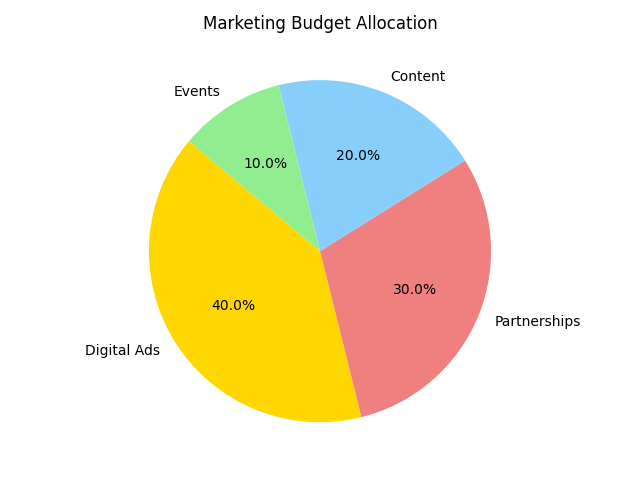
\includegraphics[width=0.8\textwidth]{images/Market budget allogation.png}
    \caption{Marketing budget allocation across digital ads, partnerships, content, and events.}
    \label{fig:marketing_budget}
\end{figure}
